\documentclass{classrep}
\usepackage[utf8]{inputenc}
\usepackage{color}
\usepackage{polski}
\usepackage{url}

\usepackage[T1]{fontenc}
\usepackage{graphicx}
\usepackage{longtable}
\usepackage{wrapfig}
\usepackage{rotating}
\usepackage[normalem]{ulem}
\usepackage{amsmath}
\usepackage{amssymb}
\usepackage{capt-of}
\usepackage{hyperref}

\DeclareUnicodeCharacter{00A0}{~}

\studycycle{Informatyka Stosowana, studia dzienne, inż I st.}
\coursesemester{IV}

\coursename{Sztuczna inteligencja i systemy ekspertowe}
\courseyear{2023/2024}

\courseteacher{Piotr Lipiński}
\coursegroup{Poniedziałek, 12:00}

\author{
  \studentinfo{Piotr Polakowski}{247768} \and
  \studentinfo{Jakub Samek}{247781} \and
  \studentinfo{Filip Kobierski}{242336}
}

\title{Zadanie Numer: Temat}

\begin{document}
\maketitle

\section{Cel}
Zadanie składa się z dwóch części: programistycznej i badawczej.
Część programistyczna stanowi napisanie programu, który będzie rozwiązywał powyższą łamigłówkę przy użyciu różnych metod przeszukiwania przestrzeni stanów stategii:
\begin{itemize}
\item \emph{wszerz} (breadth-first search);
\item \emph{w głąb} (depth-first search);
\item \emph{najpierw najlepszy}: A*, z następującymi heurystykami:
  \begin{itemize}
  \item metryką Hamminga;
  \item metryką Manhattan.
  \end{itemize}
\end{itemize}



{\color{blue}
W tej sekcji należy zamieścić zwięzły (maksymalnie dwa, trzy zdania) opis
problemu, który był rozwiązywany (uwzględnić należy zarówno część badawczą jak
i programistyczną).}

\section{Wprowadzenie}
\subsection{Algorytm BFS}
Algorytm BFS działa w taki sposób, że przeszukuje wszystkie możliwe stany idąc wszerz od węzła głównego – przeszukuje zatem wszystkie dostępne węzły na danej głębokości. Przekładając to na praktyczną implementację w „piętnastce” węzłem początkowym jest stan układanki, którą należy rozwiązać, a końcowym – układanka rozwiązana – ze wszystkimi elementami na odpowiedniej kolejności. Podczas każdej iteracji algorytmu sprawdza on dostępne możliwe ruchy, i jeżeli dane przesunięcie elementu zerowego da w rezultacie układ, który nie był do tej pory dla algorytmu znany, to staje się on kolejnym węzłem i będzie bazą do generowania możliwych przesunięć w kolejnych iteracjach. Po wygenerowaniu możliwych stanów dla danego węzła algrytm przystępuje do generowania możliwych stanów dla kolejnego węzła na tej samej głębokości, o ile jest on dostępny. Stosowana w tym przypadku jest struktura FIFO(kolejka). Algorytm kończy się w momencie, w którym napotka na stan, który odpowiada rozwiązanej układance.
\subsection{Algorytm DFS}
Algorytm DFS natomiast wyszukuje „w głąb”, czyli zamiast eksplorować wszystkie możliwe stany układanek na jednej głębokości zajmuje się jedną konkretną gałęzią – gdy znajdzie możliwy ruch w danej układance to wykonuje go, i dla układanki świeżo co zmienionej eksploruje kolejne możliwe przesunięcia. Algorytm będzie szedł „w głąb” tak długo, aż nie wyczerpie liczby możliwych stanów(co w przypadku układanki 4x4 zajęłoby bardzo dużo czasu) bądź gdy osiągnie zadaną liczbę stanów określoną manualnie w algorytmie przez programistę. Niezależnie od napotkanej przyczyny niemożności wykonania kolejnych przesunięć gdy taka sytuacja nastąpi, to algorytm cofa się do poprzedniego węzła i eksploruje kolejny możliwy stan tak samo jak w poprzednim przypadku. Algorytm DFS jest bardzo łatwy w implementacji za pomocą rekursji, natomiast można go też z powodzeniem zaimplementować iteracyjnie używając do tego celu stosu(LIFO). Algorytm kończy się, gdy znaleziona układanka będzie w takim stanie, jak układanka rozwiązana.

\subsection{Algorytm A*}
Algorytm A* jest w swoim działaniu podobny do algorytmu BFS, jednakże ma jedną sporą różnicę – nie wyznacza on „na ślepo” kolejnych możliwych sąsiadów – w naszym przypadku rozwiązań układanki, tylko posługuje się określoną metryką pozwalającą wyznaczyć najbardziej optymalny stan. W przypadku zaimplementowanego algorytmu zostały zastosowane dwie metryki:
    • Hamminga – bardzo prosta, jest to liczba pól układanki, które nie są na swoich miejscach
    • Manhattan – jest to suma odległości manhattan każdego z pól układanki od swojego miejsca docelowego
Generalnie wzór opisujący obliczanie metryki dla kolejnego stanu wygląda następująco:
\begin{equation}
f(n) = h(n) + g(n)
\end{equation}
gdzie:
\begin{itemize}
\item \(f(n)\) --- aktualny priotytet danego węzła (układanki)
\item \(h(n)\) --- wartość przyjętej metryki (w tym przypadku Hamminga lub Manhattan)
\item \(g(n)\) --- głębokość aktualnie przetwarzanego węzła
\end{itemize}

W odróżnieniu od poprzednio opisanych algorytmów A* korzysta z tzw kolejki z priorytetem – jak sama nazwa wskazuje pierwszeństwo w przetwarzaniu ma zawsze węzeł, który posiada najmniejszy w tym wypadku priorytet(mniej = lepiej). Przetwarzanie jest realizowane do momentu, gdy zostanie odnaleziony właściwy układ planszy lub wyczerpią się możliwości ruchów.


\section{Opis implementacji}
Program rozwiązujący łamigłówkę składa się z następujących plików:
\begin{itemize}
      \item main.py --- plik główny służący do wywoływania programu, przyjmujący parametry określone w zadaniu
      \item Board.py --- klasa reprezentująca obiekt układanki, pozwalająca na manupulację polami, operacje na planszy
     \item Solver.py --- klasa odpowiedzialna za rozwiązywanie układanki, zawiera metody rozwiązujące z odpowiednimi algorytmami (dfs, bfs, A*)
     \item runprog.sh --- skrypt uruchamiający przeszukiwanie układanek w trybie wsadowym
     \item runval.sh --- skrypt walidujący rozwiązania układanek zamieszczonych w plikach tekstowych
     \item exdata.sh --- skrypt pozwalający złączyć dane z wielu plików w jeden w celu wygodnego ich przetwarzania
 \end{itemize}

Skrypty w języku bash zostały pobrane ze strony przedmiotu.

Program wywołuje się poprzez plik main przekazując do niego odpowiednie parametry zgodne z tymi umieszczonymi na stronie przedmiotu, są to:

\begin{itemize}
    \item rodzaj algorytmu (bfs/dfs/astr)
    \item kolejność przeszukiwania w przypadku bfs/dfs lub metryka w przypadku A*
    \item nazwa pliku z układanką do rozwiązania
    \item nazwa pliku, do którego ma zostać zapisane rozwiązanie układanki
    \item nazwa pliku, do którego mają zostać zapisane statystyki dotyczące rozwiązania
\end{itemize}

Początkowo planowaliśmy napisać program w Javie, gdyż jest ona podobnie międzyplatformowa i kompilowana do bajtkodu.
Nawet pomimo jej większej efektywności i mniej surowych reguł składni do wykonania tego zadania wykorzystaliśmy język Python.
Ma on dynamiczne typy i jest interpretowany, czyli powolny, jednak jego kod ma mniej \emph{boilerplate} --- można wyrazić swoje myśli w kodzie mniejszą ilością znaków.
rogram napisany został w języku programowania python. 

\section{Materiały i metody}
Układanki do zbadania zostały wygenerowane przez program dostępny na stronie przedmiotu. Każda z układanek została zbadana każdym z algorytmów przy każdej możliwej kombinacji parametrów wywołania. 

Do przeprowadzenia badania wszystkich wygenerowanych układów łamigłówek został wykorzystany skrypt dostępny na stronie przedmiotu. Umożliwiał on przetestowanie wszyskich możliwych kombinacji – wywoływał on w naszym przypadku program z odpowiednimi, ustandaryzowanymi wcześniej parametrami wywołania tak, aby zbadać wszyskie możliwe stany. Po uruchomieniu skryptu należało odczekać znaczną ilość czasu, aby ten wygenerował wszystkie niezbędne rozwiązania, które były dwoma rodzajami plików tekstowych zawierających:

\begin{itemize}
    \item plik 1: długość znalezionego rozwiązania, ciąg liter odpowiadający kolejności przesunięć, które prowadziły do rozwiązania układanki
    \item plik 2: długość znalezionego rozwiązania, liczba stanów odwiedzonych, liczba stanów przetworzonych, maksymalna osiągnięta głębokość, czas wykonania(w ms)
\end{itemize}

Wynikiem wykonania programu było otrzymanie bardzo dużej liczby plików z danymi. W celu wygodnego ich przetwarzania został wykorzystany kolejny skrypt ze strony przedmiotu – exdata.sh, wyjście skryptu za pomocą potoku zostało przekierowane do pliku tekstowego, dzięki czemu można było na podstawie pojedynczego pliku utworzyć odpowiednie wykresy i analizować otrzymane w wyniku przetwarzania rozwiązań układanek dane.

\section{Wyniki}

\begin{figure}[p] \centering
 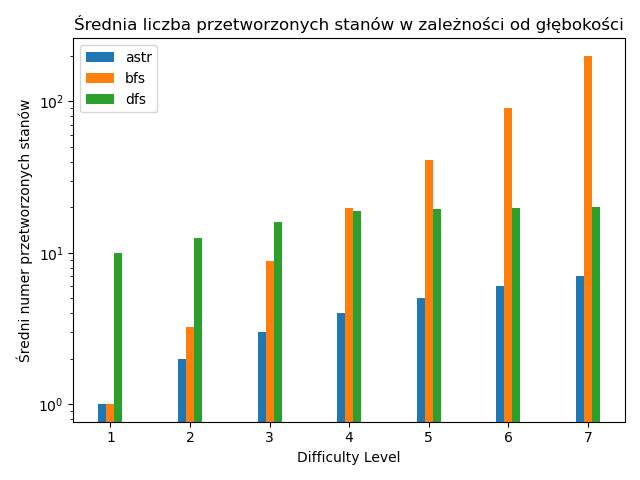
\includegraphics[width=0.9\linewidth]{./pic/glob_proc_c_vs_diff.png}
 \caption{Globalnie: trudność a przetworzone stany}
\end{figure}
\begin{figure}[p] \centering
 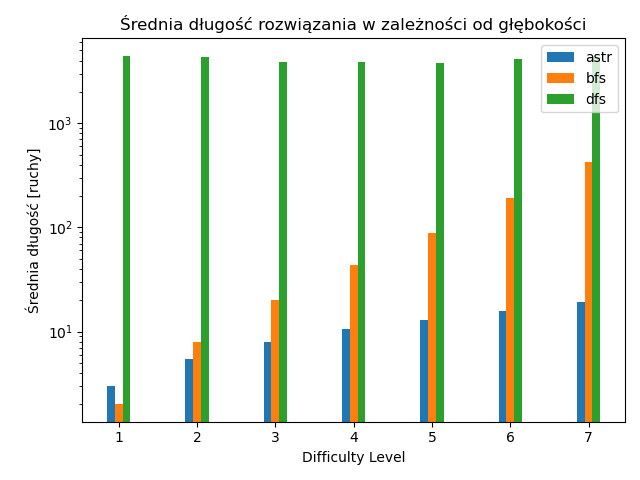
\includegraphics[width=0.9\linewidth]{./pic/glob_sol_len_vs_diff.png}
 \caption{Globalnie: trudność a długość rozwiązania}
\end{figure}
\begin{figure}[p] \centering
 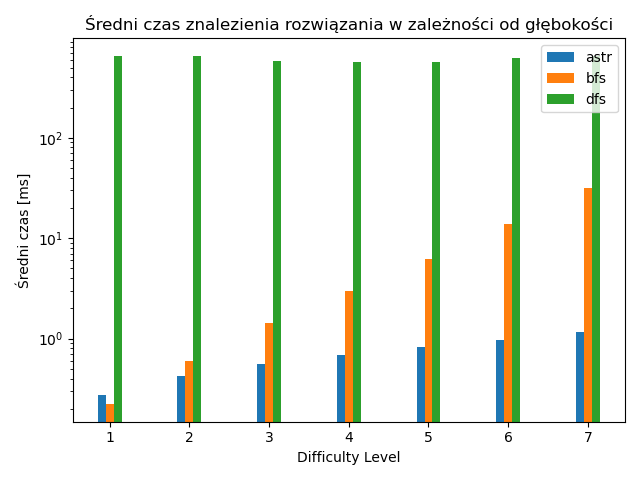
\includegraphics[width=0.9\linewidth]{./pic/glob_time_vs_diff.png}
 \caption{Globalnie: trudność a czas rozwiązania}
\end{figure}
\begin{figure}[p] \centering
 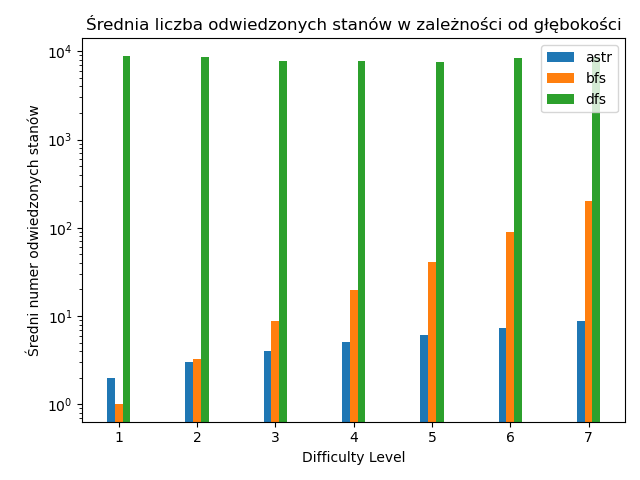
\includegraphics[width=0.9\linewidth]{./pic/glob_vstd_c_vs_diff.png}
 \caption{Globalnie: trudność a odwiedzone stany}
\end{figure}

\begin{figure}[p] \centering
 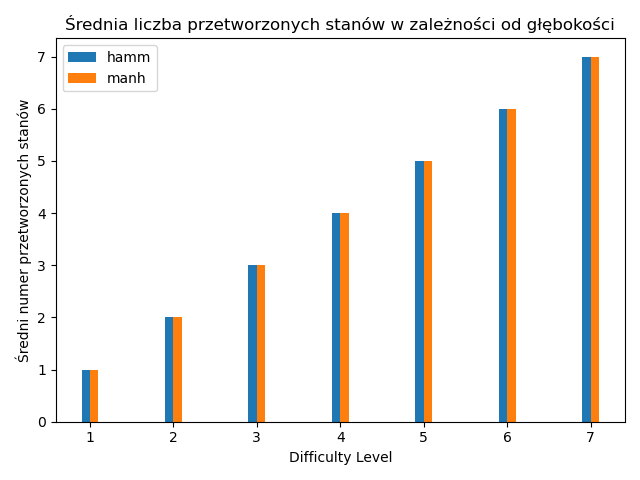
\includegraphics[width=0.9\linewidth]{./pic/astr_proc_c_vs_diff.png}
 \caption{A*: trudność a przetworzone stany}
\end{figure}
\begin{figure}[p] \centering
 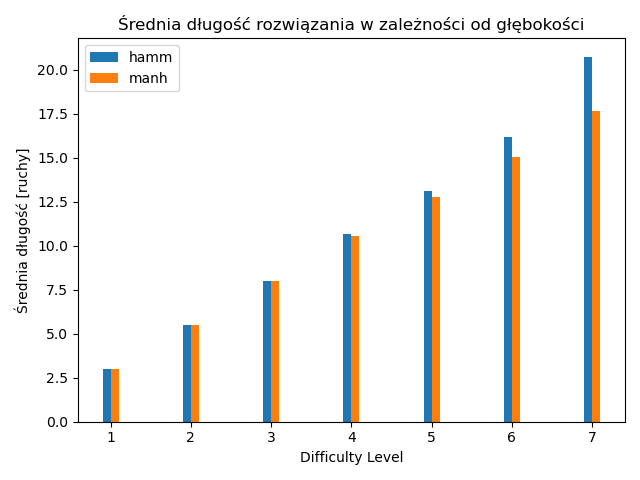
\includegraphics[width=0.9\linewidth]{./pic/astr_sol_len_vs_diff.png}
 \caption{A*: trudność a długość rozwiązania}
\end{figure}
\begin{figure}[p] \centering
 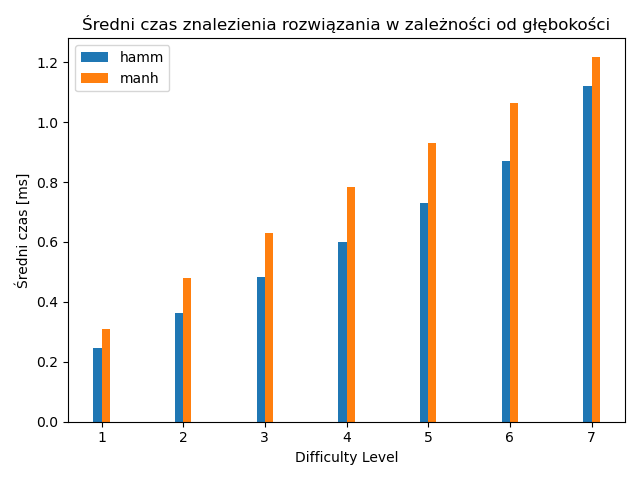
\includegraphics[width=0.9\linewidth]{./pic/astr_time_vs_diff.png}
 \caption{A*: trudność a czas rozwiązania}
\end{figure}
\begin{figure}[p] \centering
 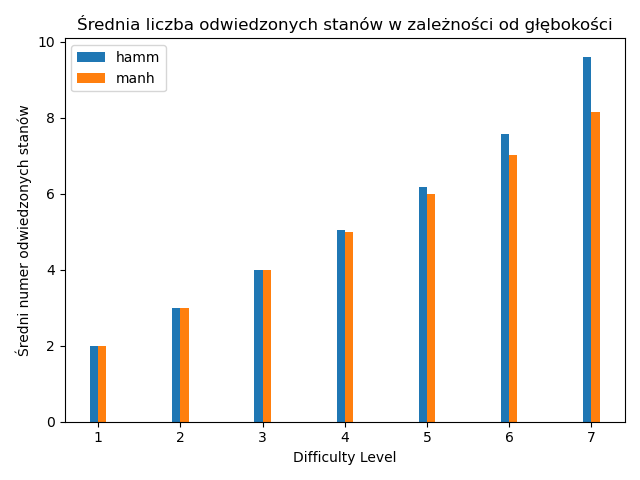
\includegraphics[width=0.9\linewidth]{./pic/astr_vstd_c_vs_diff.png}
 \caption{A*: trudność a odwiedzone stany}
\end{figure}

\begin{figure}[p] \centering
 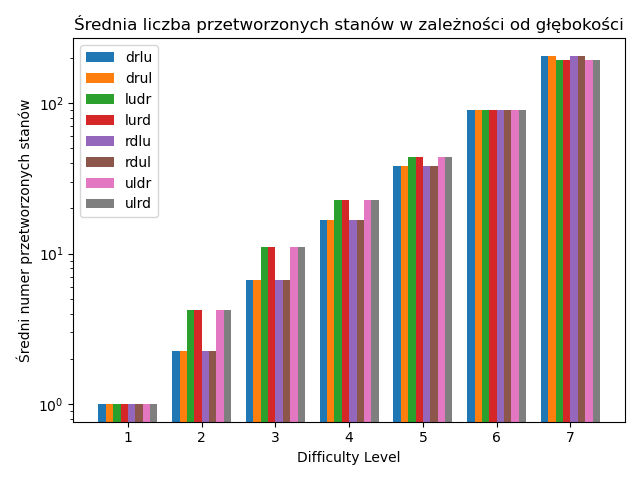
\includegraphics[width=0.9\linewidth]{./pic/bfs_proc_c_vs_diff.png}
 \caption{BFS: trudność a przetworzone stany}
\end{figure}
\begin{figure}[p] \centering
 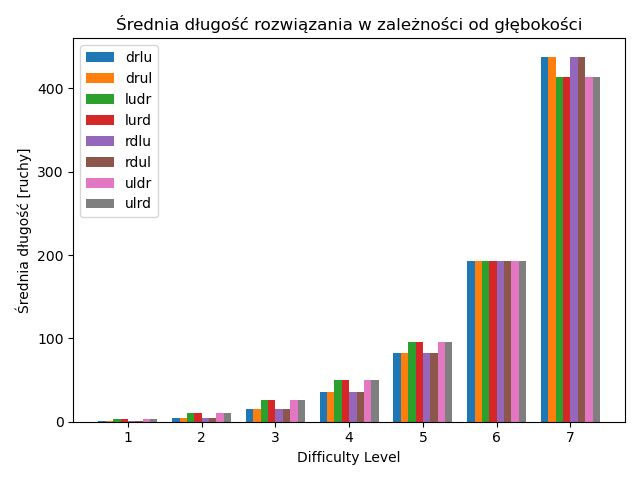
\includegraphics[width=0.9\linewidth]{./pic/bfs_sol_len_vs_diff.png}
 \caption{BFS: trudność a długość rozwiązania}
\end{figure}
\begin{figure}[p] \centering
 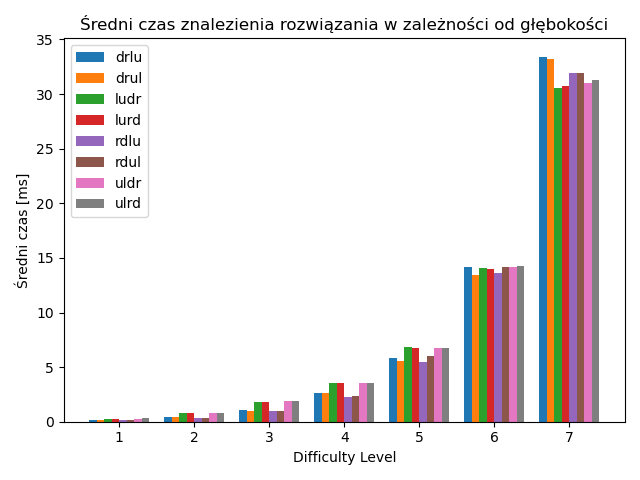
\includegraphics[width=0.9\linewidth]{./pic/bfs_time_vs_diff.png}
 \caption{BFS: trudność a odwiedzone stany}
\end{figure}
\begin{figure}[p] \centering
 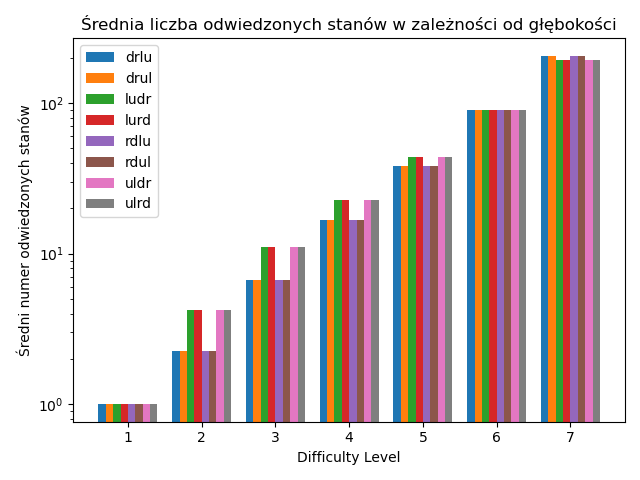
\includegraphics[width=0.9\linewidth]{./pic/bfs_vstd_c_vs_diff.png}
 \caption{BFS: trudność a czas rozwiązania}
\end{figure}

\begin{figure}[p] \centering
 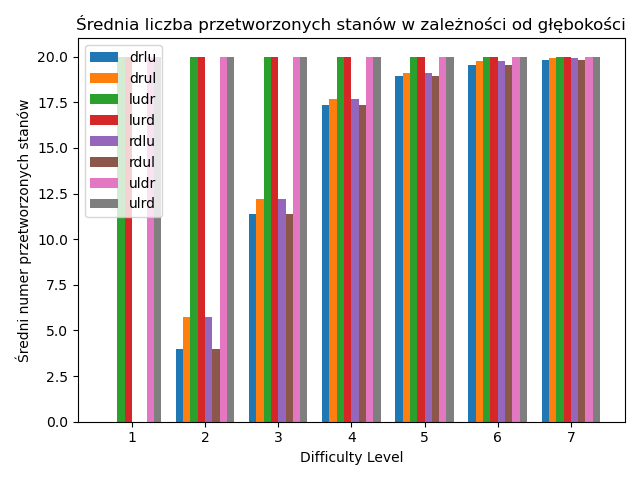
\includegraphics[width=0.9\linewidth]{./pic/dfs_proc_c_vs_diff.png}
 \caption{DFS: trudność a przetworzone stany}
\end{figure}
\begin{figure}[p] \centering
 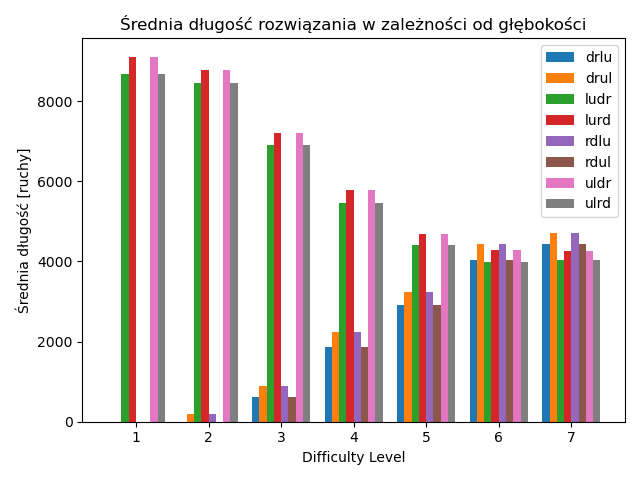
\includegraphics[width=0.9\linewidth]{./pic/dfs_sol_len_vs_diff.png}
 \caption{DFS: trudność a długość rozwiązania}
\end{figure}
\begin{figure}[p] \centering
 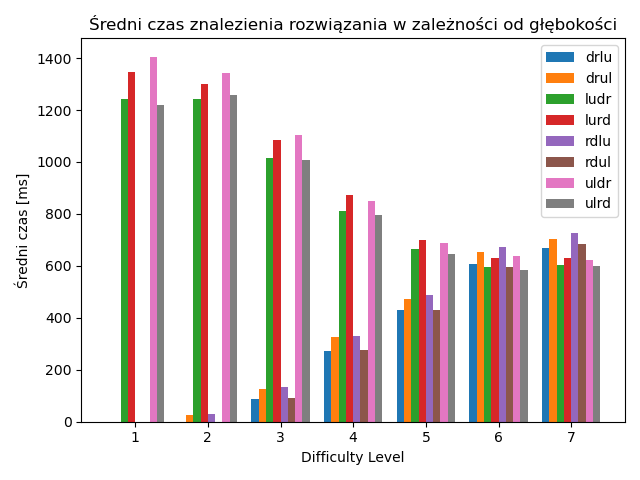
\includegraphics[width=0.9\linewidth]{./pic/dfs_time_vs_diff.png}
 \caption{DFS: trudność a czas rozwiązania}
\end{figure}
\begin{figure}[p] \centering
 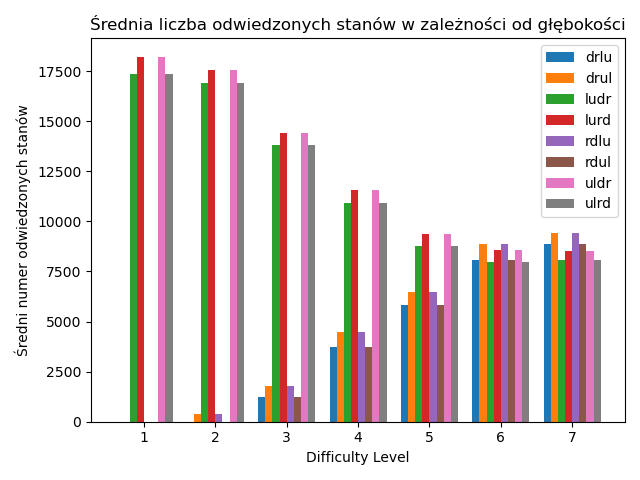
\includegraphics[width=0.9\linewidth]{./pic/dfs_vstd_c_vs_diff.png}
 \caption{DFS: trudność a odwiedzone stany}
\end{figure}

\section{Dyskusja}
\subsection{Globalnie}
W przytłaczającej większości przypadków algrytm A* był najlepszy pod każdym względem.
Przy bardzo prostych układankach czasami BFS szybciej znajdywał rozwiązanie, jednak różnicza jest niewielka

\subsection{Heurystyki A*}
Nie można jednonacznie stwiedzić czy heurystyka Hamminga czy Manhattan są lepsze.
Obydwa do rzwiązania potrzebują przetworzyć taką samą liczbę stanów, jednak Hamminga odwiedza ich więcej przy trudniejszych ukłądankach i  jest szybszy.

\subsection{Strategie BFS i DFS}

\section{Wnioski}
Algorytm A* okazał się najszybszy, ale w teorii nie zawsze może dać rozwiązanie w przypadku bardziej skomplikowanych układanek. W przypadku tego algorytmu w naszych eksperymentach czas wykonania programu jak i ilosć odwiedzonych stanów pozostawała na bardzo niskim poziomie w miarę zwiększania się trudności poszczególnych układanek. 

Algorytm bfs jest w teorii algorytmem, który zawsze znajdzie rozwiązanie, nie zawsze jednak w tak optymalnym czasie, jak algorytm wykorzystujący heurystyki. W tym przypadku czas rozwiązywania układanek przez algorytm bfs był na niskim poziomie, rozwiązane zostały wszysktie układanki. BFS jest algorytmem optymalnym, gdy nie znamy rozkładu danych i chcemy mieć pewność uzyskania rozwiązania.

DFS okazał się w tym zestawieniu najwolniejszy, i choć rozwiązał wszystkie zadane układanki, robił to z największą liczbą przetworzonych i odwiedzonych stanów, a co za tym idzie z największym czasem wykonywania. Algorytm ten jeżeli źle, nieoptymalnie będzie wybierał kolejne węzły znacznie wydłuża swój czas wykonania i liczbę przetwarzanych/odwiedzanych stanów. Sytuacja wygląda inaczej, gdy znamy rozkład danych – wtedy DFS przy dobraniu optymalnych węzłów przetwarzających może okazać się naprawdę wydajnym rozwiązaniem.
\begin{thebibliography}{0}
  \bibitem{l2short} T. Oetiker, H. Partl, I. Hyna, E. Schlegl.
    \textsl{Nie za krótkie wprowadzenie do systemu \LaTeX2e}, 2007, dostępny online.
\end{thebibliography}
\end{document}
